\documentclass{beamer}

\usetheme{Frankfurt}
\usecolortheme{dolphin}

\usepackage{amsmath, amssymb, amsfonts, tikz}
\usepackage[utf8]{inputenc}
\usepackage[T1]{fontenc}
\usepackage[english]{babel}

\DeclareTextFontCommand{\emph}{\bfseries}

\hypersetup{pdfstartview={Fit}}

\author{Alex J. Best}
\institute{WMS Talks}
\date{4/2/2014}
\title{Riemann Hypotheses}

\begin{document}

\section{Introduction}

\frame{\titlepage}

\begin{frame}
\frametitle{In this talk:}
\note{will talk first about the riemann zeta and millenium prize problem associated with it, and then about functions defined in similar ways to the classical zeta and the meanings of associated hypotheses for them.}
\tableofcontents
\note{apologies no fractals?} % Maybe too hard?!
\end{frame}

\section{The original hypothesis}

\begin{frame}{The Riemann zeta function: Euler's work}
A brief history of $\zeta$:
\begin{itemize}
\item In 1735 Euler solves the \emph{Basel problem} by finding that
\[\sum_{n=1}^{\infty} \frac{1}{n^2} = \frac{\pi^2}{6}.\]
\pause \item He also discovered more general formulae for $\sum_{n=1}^{\infty} n^{-2k}$ in terms of the Bernoulli numbers $B_{2k}$ for all natural $k$.
\note{nowadays we see this as evaluating $\zeta(2)$.}
\pause \item In fact, a nice form for \[\sum_{n=1}^{\infty} n^{-2k-1},\] is still unknown today.
\end{itemize}
\end{frame}

\begin{frame}{The Riemann zeta function: Along comes Riemann}
\begin{columns}
\begin{column}{.575\textwidth}
A brief history of $\zeta$:
\begin{itemize}
\item In 1859 Bernhard Riemann, a well known analyst, publishes a paper on his work counting the primes using analysis.
\item<2-> In the paper he considers
\[
\zeta(s) = \sum_{n=1}^{\infty} \frac{1}{n^s}.
\]
\note{this is the only paper on number theory he every publishes, a thankyou to the berlin academy for accepting him as a corresponding member, miracle he published it all given its sketchy nature he rarely published unpolished work}
\item<3-> Here the notation $\zeta$ for this function is used for the first time.
\item<4-> Along the way he (essentially) makes four hypotheses.
\note{these are not the hypotheses we are going to talk about, bar one, which we will get to in a minute. Riemann himself disregarded the hypothesis and seemingly barely did any work on it after the paper was published.}
\end{itemize}
\end{column}
\begin{column}{.425\textwidth}
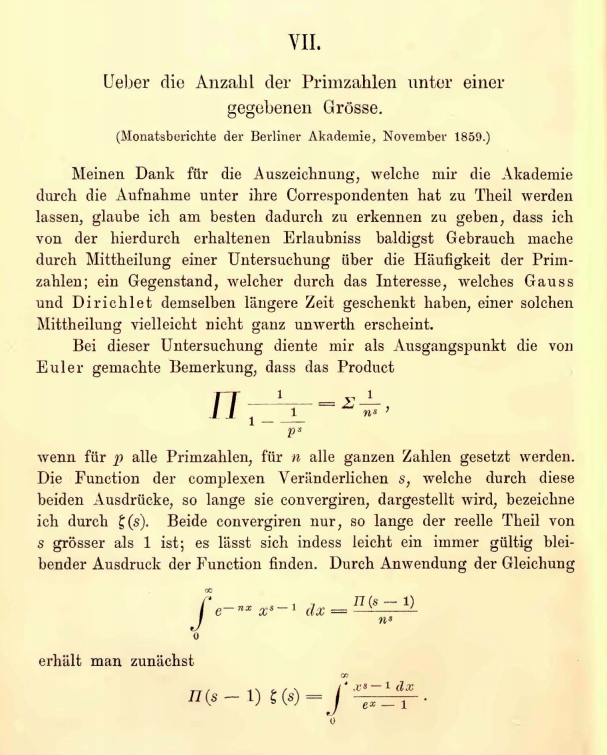
\includegraphics[width=\textwidth]{img/ueber}
\end{column}
\end{columns}
\end{frame}

\begin{frame}{The Riemann zeta function: What Riemann did}
In his work Euler had (more or less) found that 
\[\zeta(s) = \sum_{n=1}^{\infty}\frac{1}{n^s} = \prod_{p \text{ prime}}\frac{1}{1-p^s}.\]
\pause In his paper Riemann uses this to take the function $\zeta\colon \{\sigma + it \in\mathbb{C}\mid \sigma > 1\} \to \mathbb{C}$ and extend it to all of $\mathbb{C}$.
\pause He defines an \emph{analytic} function from $\mathbb{C} \to \mathbb{C}$ which matches the series definition given above when the series converges (when $\operatorname{Re}(s) > 1$).
\pause Riemann also discovers a \emph{functional equation} for the zeta function by showing that
\[ \pi^{-s/2} \Gamma\left(\frac{s}{2}\right)\zeta(s) = \pi^{-(1-s)/2} \Gamma\left(\frac{1-s}{2}\right) \zeta(1-s).\]
\note{details of this aren't important to us, but this sort of self similarity is a feature in common of many of the functions we will meet.}
\end{frame}

\begin{frame}{The Riemann zeta function: What does it look like?}
\begin{center}
\only<1>{$f(s) = s$:\\[0.7em]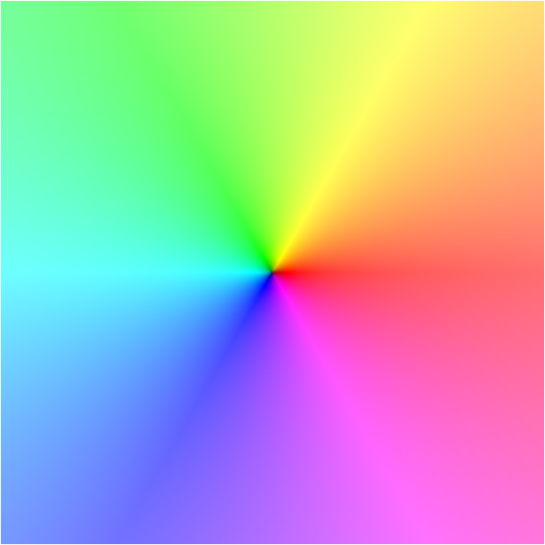
\includegraphics[height=0.75\textheight]{img/id}}
\only<2>{$\zeta(s)$:\\[0.7em]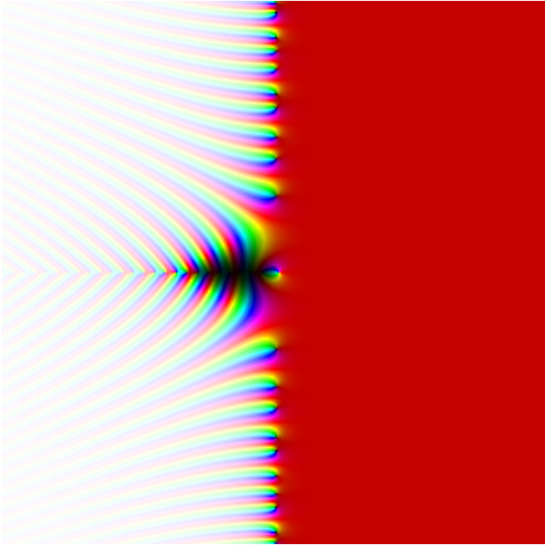
\includegraphics[height=0.75\textheight]{img/wide}}
\only<3>{$\zeta(s)$:\\[0.7em]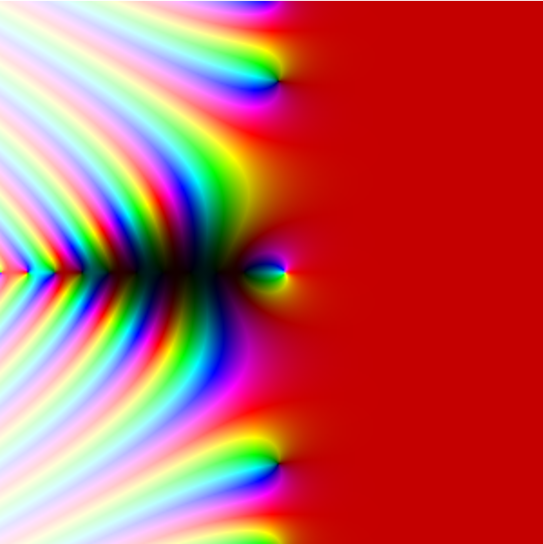
\includegraphics[height=0.75\textheight]{img/close}}
\only<4>{$\zeta(s)$:\\[0.7em]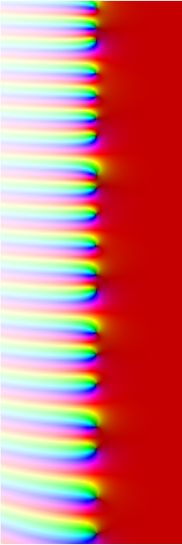
\includegraphics[angle=90,width=\textwidth]{img/zeroes}}
\end{center}
\end{frame}

\begin{frame}{The Riemann zeta function: The hypothesis}
The zeta function has ``trivial'' zeroes at the negative even integers, but also ``non-trivial'' zeroes lying on the line $\operatorname{Re}(s) = \frac{1}{2}$.
\pause\begin{block}{The Riemann Hypothesis (RH)}
All non-trivial zeroes of the Riemann zeta function lie on the \emph{critical line}
\[\left\{s\in \mathbb{C} \colon \operatorname{Re}(s) = \frac{1}{2}\right\}.\]
\end{block}\note{Riemann himself couldn't make nice plots like we can and instead defined another function with the same non-trivial zeroes as the zeta}
\pause {\bf Why do we care?} \note{Riemann considered it very likely that all the zeroes of the function lay on the critical line, but didn't seem particularly interested in trying to prove it}
\begin{itemize}
\pause \item It is a natural function to consider, and knowing the zeroes of a complex function are key to understanding it. \note{those who came to bartels talk on what is an elliptic curve and why should I care, the take away there was really, its the least complicated class of curve thats complicated enough that we dont understand it, and I guess you could say something similar about riemann's zeta}
\pause \item The location of the zeroes of $\zeta(s)$ relates in a strong way to the distribution of the primes.
\end{itemize}
\end{frame}

\begin{frame}{The Riemann zeta function: Why number theorists care}
\note{the primes are the basic building blocks of the natural numbers, so knowing their behaviour is very useful. It is pretty much impossible given a prime to tell when the next one occurs, however it is possible to work out formulae that approximate how the number of primes grows as we move further through the naturals. In fact Riemanns paper was entitled on the number of primes less than a given magnitude.}
\begin{block}{The prime counting function $\pi(x)$}
We define
\[ \pi(x) = |\{p \in \mathbb{N} \colon p \text{ prime, }p\le x\}|.\]
\end{block} \note{Riemanns paper initiated use of complex analysis to study this function.}

\pause Gauss noticed that $\pi(x)$ is approximated well by
\[\operatorname{Li}(x) = \int_{0}^{x} \frac{\mathrm{d} t}{\log t}\]
which was later confirmed by some of Chebyshev's work.

\pause The Riemann hypothesis is actually equivalent to the statement that there exists $c_2 > c_1 > 0$ such that
\[\operatorname{Li}(x) + c_1\sqrt{x}\log(x) \le \pi(x) \le \operatorname{Li}(x) + c_2\sqrt{x}\log(x)\]
eventually.
These are the best possible bounds! \note{Shown by Koch, of snowflake fame}
\note{even though RH is unsolved, other properties of zeta are useful, for example no zeroes on Re = 1 gives classic prime number theorem pi(x) ~ x/log x.}
\end{frame}

\note{I've talked for some time now about RH so I suppose I should move onto some others}

\section{Zeta functions for graphs}
\note{now time for something completely different, the links should become clear shortly.}

\begin{frame}{Expander graphs}
\begin{columns}
\begin{column}{.618\textwidth}

Suppose we want to design a communications network (for computers, people, phones, etc.) by linking together $n$ entities with wires, such that each object has only $k$ wires from it (this is called \emph{$k$-regular}).

\pause We shall call our entities \emph{nodes} and wires \emph{edges}, as in graph theory.

~\\
\note{There are several properties of such a network we could want}
\pause For today we will think of our goal as the following:

If we split our network into two nonempty parts (a partition) there should be lots of edges between the two halves. \note{so lots of messages can get through simultaneously}
\end{column}
\begin{column}{.3819\textwidth}

\tikzstyle{every node}=[circle, draw, fill=black!50,
                        inner sep=0pt, minimum width=4pt]
\pause
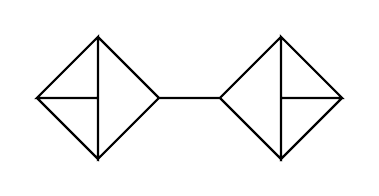
\begin{tikzpicture}[thick,scale=0.775]%
        \draw (0,0) node{} -- (1,1) node{} -- (2,0) node{}
 -- (3,0) node{} -- (4,1) node{} -- (5,0) node{} -- (4,-1) node{}
 -- (4,0) node{} -- (5,0) node{} -- (4,1) node{} -- (4,0) node{}
 -- (4,-1) node{} -- (3,0) node{} -- (2,0) node{} -- (1,-1) node{}
 -- (1,0) node{} -- (1,1) node{} -- (0,0) node{} -- (1,0) node{}
 -- (1,-1) node{} -- (0,0) node{};
\end{tikzpicture}
\pause
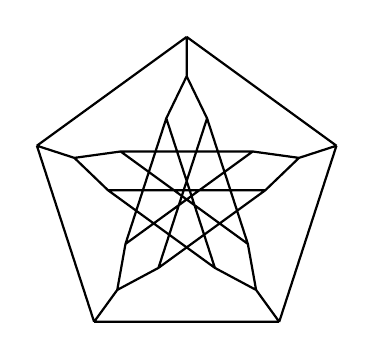
\begin{tikzpicture}[thick,scale=0.5]%
    \draw \foreach \x in {18,90,...,306} {
        (\x:4) node{} -- (\x+72:4)
        (\x:4) -- (\x:3) node{}
        (\x:3) -- (\x+15:2) node{}
        (\x:3) -- (\x-15:2) node{}
        (\x+15:2) -- (\x+144-15:2)
        (\x-15:2) -- (\x+144+15:2)
};
\end{tikzpicture}
\end{column}
\end{columns}
\note{many applications in CS of course, and not just practical network stuff more theoretical ideas too, recently (~10 years) these ideas have found more uses within mathematics.}
\end{frame}

\begin{frame}{The spectrum}
Given such a graph $G$ we can fix a numbering of the vertices and form:
\begin{block}{The adjacency matrix}
Is an $n\times n$ matrix $A_G = (a_{ij})$ of 1's and 0's given by
\[a_{ij} = 1 \iff \text{ there is an edge between vertex $i$ and vertex $j$}.\]
\end{block}
\note{do an example from the previous slide}
\pause What are the eigenvalues of this matrix?\note{talk through ex, clearly have k, d is always one, not so interesting, so we instead look at this so called second eigenvalue} 
\pause So we define $\lambda(G)$ to be the next largest eigenvalue after $d$, i.e.
\[\lambda(G) = \max_{|\lambda_i| < d} |\lambda_i|.\]

\end{frame}

\begin{frame}{Ramanujan graphs}
It turns out that for fixed $\epsilon$ only finitely many graphs do not satisfy 
\[\lambda(G) \ge 2\sqrt{k-1} - \epsilon.\]
\pause This set of graphs must be pretty special, so we name them
\begin{block}{Ramanujan graphs}
A graph $G$ as above which satisfies
\[\lambda(G) \le 2\sqrt{k-1}.\]
\end{block}
These are highly optimal from our point of view!
\pause Ramanujan graphs are only known to exist for $k = p^n + 1$.
\end{frame}

% Sarnak wolf prize
\begin{frame}{The Ihara zeta function}
Take a graph $G$ as described above ($k$-regular for some $k$, finite and connected).
We define:
\begin{block}{A prime in $G$}

\end{block}
% Length!!
\pause \begin{block}{The Ihara zeta function of $G$}
\[\zeta_G(u) = \prod_{P\text{ a prime of } G} \left(1-u^{\nu(p)}\right)^{-1}.\]
\end{block}
\end{frame}

\begin{frame}
The Ihara zeta function has slightly different behaviour than the classical zeta, there are poles instead of zeroes!
\pause So we might conjecture
\begin{block}{RH for graphs}

\end{block}
\pause Is this true?
\begin{block}{Theorem}
A graph $G$ satisfies the RH for graphs $\iff$ it is Ramanujan.
\end{block}
\end{frame}

\section[More zetas]{More assorted zetas}

% Do geodesics

\begin{frame}{What else has a zeta function?}
\note{maybe a better question is what doesn't!}
\begin{itemize}
\pause\item Dynamical systems, the Ruelle zeta is actually a generalisation of the Ihara zeta function we just saw.
\pause\item Function fields (that the analogue of RH is true was proved by Andr\'e Weil in the 40's).
\pause\item Curves over finite fields.
\pause\item Fractal strings.
\pause\item Schemes (over finite type over $\mathbb{Z}$).
\end{itemize}
\end{frame}

\section[Number theory again]{Back to number theory}
\note{didn't want to talk about number theory so much as I wanted to focus more on why you might care about zeta functions even if you don't care about the structure of the primes.}
\begin{frame}{The Dedekind zeta function}
Richard Dedekind (1831--1916) wanted to use analysis to study more general fields called number fields.

\pause \begin{block}{Number fields}
A \emph{number field} is a field that is also a finite dimensional $\mathbb{Q}$-vector space.
\end{block}

\pause e.g. $\{a+bi\mid a,b\in\mathbb{Q}\}$, \pause $\{a+b\sqrt{2}\mid a,b\in\mathbb{Q}\}$, \pause $\{a+b\sqrt{2} +c\sqrt{3}+d\sqrt{2}\sqrt{3}\mid a,b,c,d\in\mathbb{Q}\}$.

\pause In a general number field the idea of a prime element doesn't work out so well, however if we consider nice subgroups of the field (ideals of the ring of integers) then everything works out well, so we should deal with ideals instead of elements!
\pause For example we  have unique factorisation of ideals into prime ideals.
\end{frame}

\begin{frame}{The Dedekind zeta function}
So Dedekind defined for a number field $K$
\begin{block}{The Dedekind zeta function}\note{what do we want to write here}
\[\zeta_K(s) = \pause \sum_{I\subset \mathcal{O}_K} \frac{1}{N(I)^s}\]
where $N(I)$ is the \emph{norm} of $I$ ($ = |\mathcal{O}/I|$). \note{its size}
\end{block}
\pause $\mathbb{Q}$ is a number field too, and it turns out that the ideals of $\mathbb{Q}$ correspond one to one with the set of natural numbers.
We then have $N((n)) = |\mathbb{Z}/(n)| = n$.
\pause Therefore
\[\zeta(s) = \zeta_\mathbb{Q}(s).\]\note{the Dedekind zeta is a direct generalisation of our original zeta}
\note{The analogue of the Riemann hypothesis for the Dedekind zeta is exactly the same.}
\pause A proof of these hypotheses for all number fields (known as the \emph{extended} Riemann hypothesis) would give approximations for the number of prime ideals of bounded norm, exactly the same as for the original hypothesis.
\note{in fact we have an Euler product for this function too! and of course its RH tells us about the primes of the number field. don't get into as not so many people know ant!}
\end{frame}

\section{Conclusion}
\begin{frame}{Closing remarks}
\begin{itemize}
\item Zeta functions can be used to pack up lots of useful information into one big package (a complex function).
\pause\item The properties of this package can tell us about the objects we started with.
\pause\item We can also see links between different objects via their zeta functions.
\pause\item Due to the abundant computational evidence (over ten trillion non-trivial zeroes found so far, all on the critical line) a huge number of papers have been written that assume the Riemann hypothesis is true.
So a proof of the (generalised) hypothesis would imply hundreds of other results true also.
\end{itemize}
\end{frame}

\begin{frame}{Sources used}
I used some of the following when preparing this talk, and so they are possibly good places to look to learn more about the topic:
\begin{enumerate}
\item ``What is... an expander?'' -- Peter Sarnak
\item ``Problems of the Millennium: The Riemann Hypothesis'' -- Peter Sarnak
\item ``Problems of the Millennium: The Riemann Hypothesis'' (Official Millennium prize problem description) -- Enrico Bombieri
\item ``Zeta Functions of Graphs: A Stroll through the Garden'' -- Audrey Terras
\item Wikipedia -- Enough said
\item http://graphtheoryinlatex.blogspot.com/ -- Pretty pictures
\item ``Fractal Geometry, Complex Dimensions and Zeta Functions'' -- Lapidus and van Frankenhuijsen (not used in talk but still cool)
\end{enumerate}
\end{frame}

\end{document}


